% Provenance (never printed): cycle 2 "Questionner le monde" (states of water in
% weather phenomena; daily observation), see sources/book1/PROVENANCE.md.
% Book 1, grade 1, chapter 1. No real-world number in this chapter.
\chapter{Kijken naar het weer}\label{ch:g1:watching-the-weather}

Het is vroeg in de ochtend. Lena wordt wakker, klimt op de stoel bij het
raam van haar slaapkamer en kijkt naar buiten. De lucht is grijs. Kleine
waterdruppels lopen langs het glas naar beneden. De daken aan de overkant
zijn nat en glimmen, en de boom in de tuin druppelt.

``Wat zal ik vandaag aantrekken?'' vraagt ze.

Om dat te weten heeft Lena geen boek en geen apparaat nodig. Ze hoeft
alleen uit het raam te kijken. Het raam is haar eerste weerstation.

\begin{omfigure}
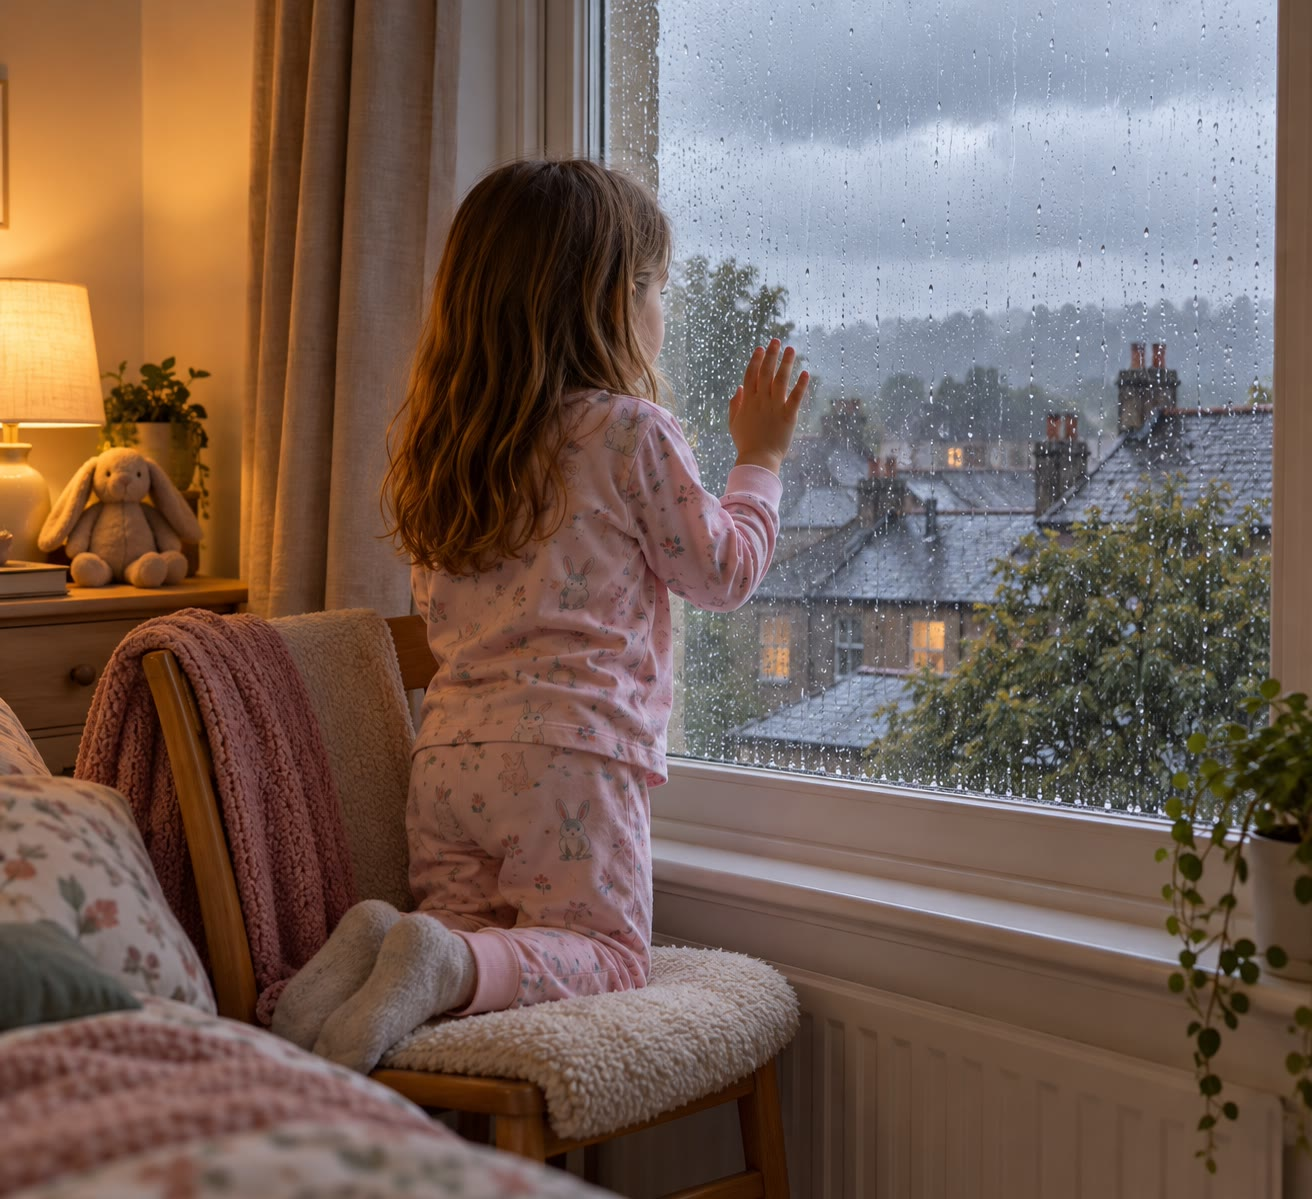
\includegraphics[width=0.72\linewidth]{images/book1/ai/g1-rainy-window.jpg}

{\small Een grijze, regenachtige ochtend, gezien door een raam.}
\end{omfigure}

\begin{recall}
Elke ochtend komt de Zon op en begint de dag; elke avond gaat ze onder en
wordt het nacht. In de natuurkundeboeken heb je gezien waarom de dag en de
nacht elkaar afwisselen. In dit hoofdstuk kijken we naar iets anders dat
steeds verandert: het \omterm{def:g1:watching-the-weather:weather}{weer}.
\end{recall}

\section{Wat is het weer?}

Als we naar buiten gaan, voelen we de lucht op ons gezicht. Die kan warm
of koud zijn. Ze kan stil zijn, of ze duwt tegen ons haar en onze kleren:
dan waait het. We kijken omhoog. De hemel kan blauw en helder zijn, of vol
wolken. Soms valt er regen uit de wolken, soms sneeuw. Dat alles samen is
het \omterm{def:g1:watching-the-weather:weather}{weer}.

\begin{definition}[Weer]\label{def:g1:watching-the-weather:weather}
Het \emph{weer}\index{weer} is hoe de lucht en de hemel zijn op één
plek en op één moment: zonnig of bewolkt, droog of met regen of sneeuw,
windstil of winderig, warm of koud.
\end{definition}

Om het \omterm{def:g1:watching-the-weather:weather}{weer} te beschrijven, beantwoorden we een paar eenvoudige vragen:
\begin{enumerate}
  \item \textbf{Hoe ziet de hemel eruit?} Is hij blauw en schijnt de Zon?
        Zijn er een paar wolken, of is alles grijs?
  \item \textbf{Valt er iets uit de lucht?} Regen? Sneeuw? Niets?
  \item \textbf{Waait het?} Bewegen de bladeren van de bomen? Wappert er
        een vlag?
  \item \textbf{Is het warm of koud?} Hebben we een jas nodig?
\end{enumerate}

\begin{omfigure}
\begin{minipage}[b]{0.49\linewidth}\centering
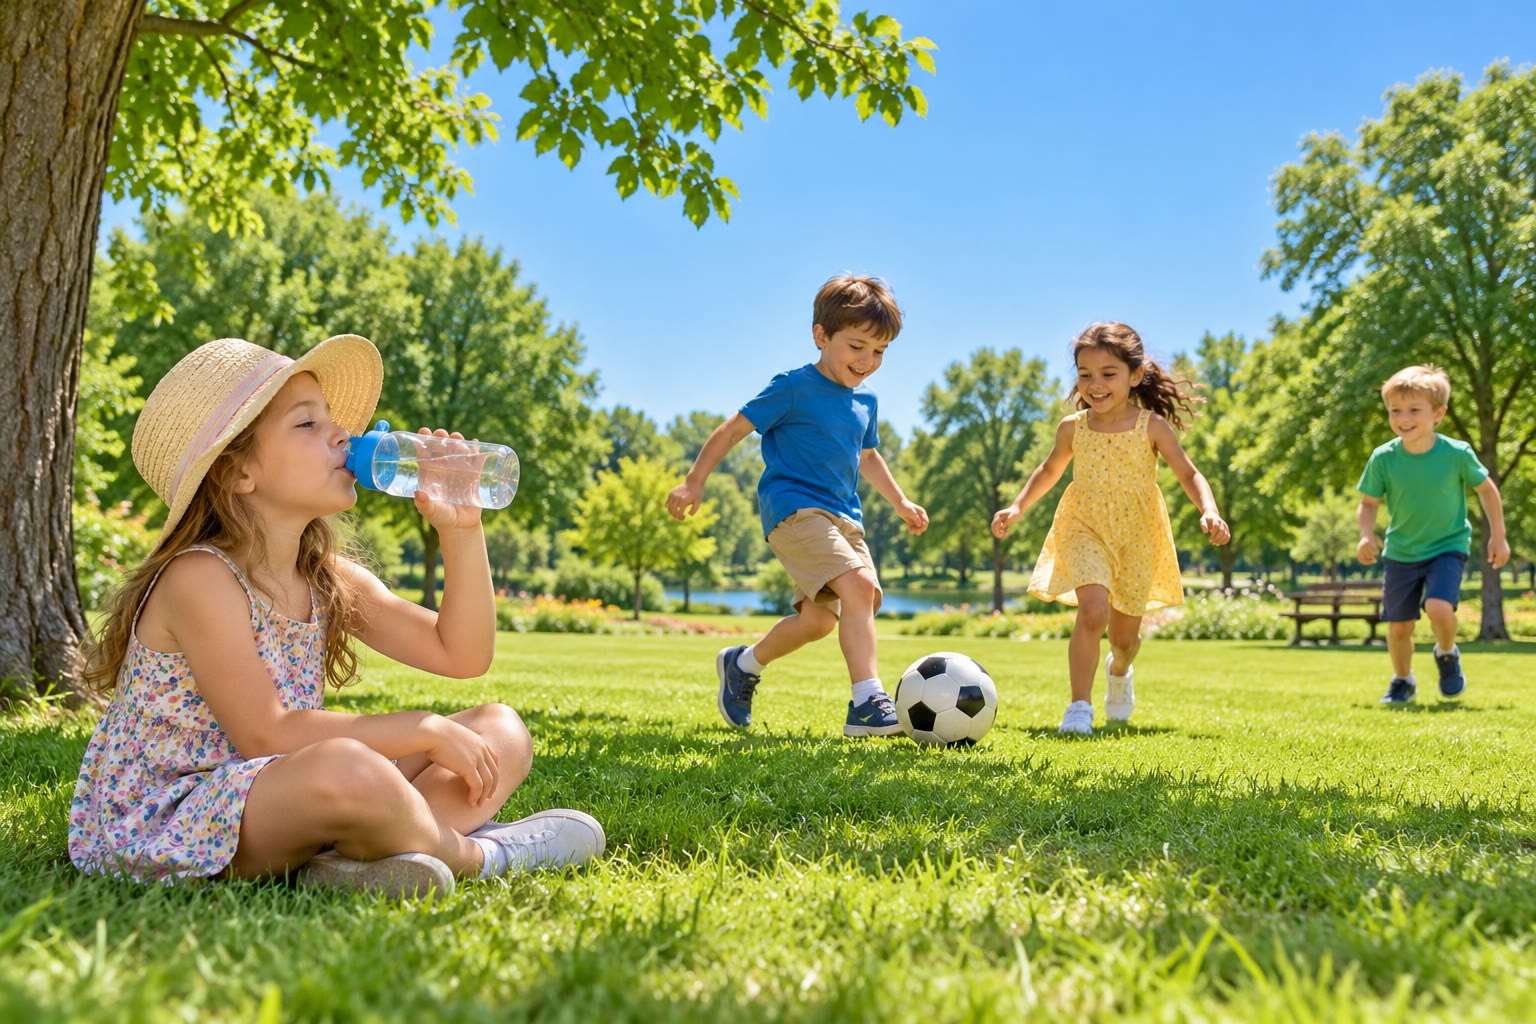
\includegraphics[width=\linewidth]{images/book1/ai/g1-sunny-park.jpg}

{\small Zonnig en warm.}
\end{minipage}\hfill
\begin{minipage}[b]{0.49\linewidth}\centering
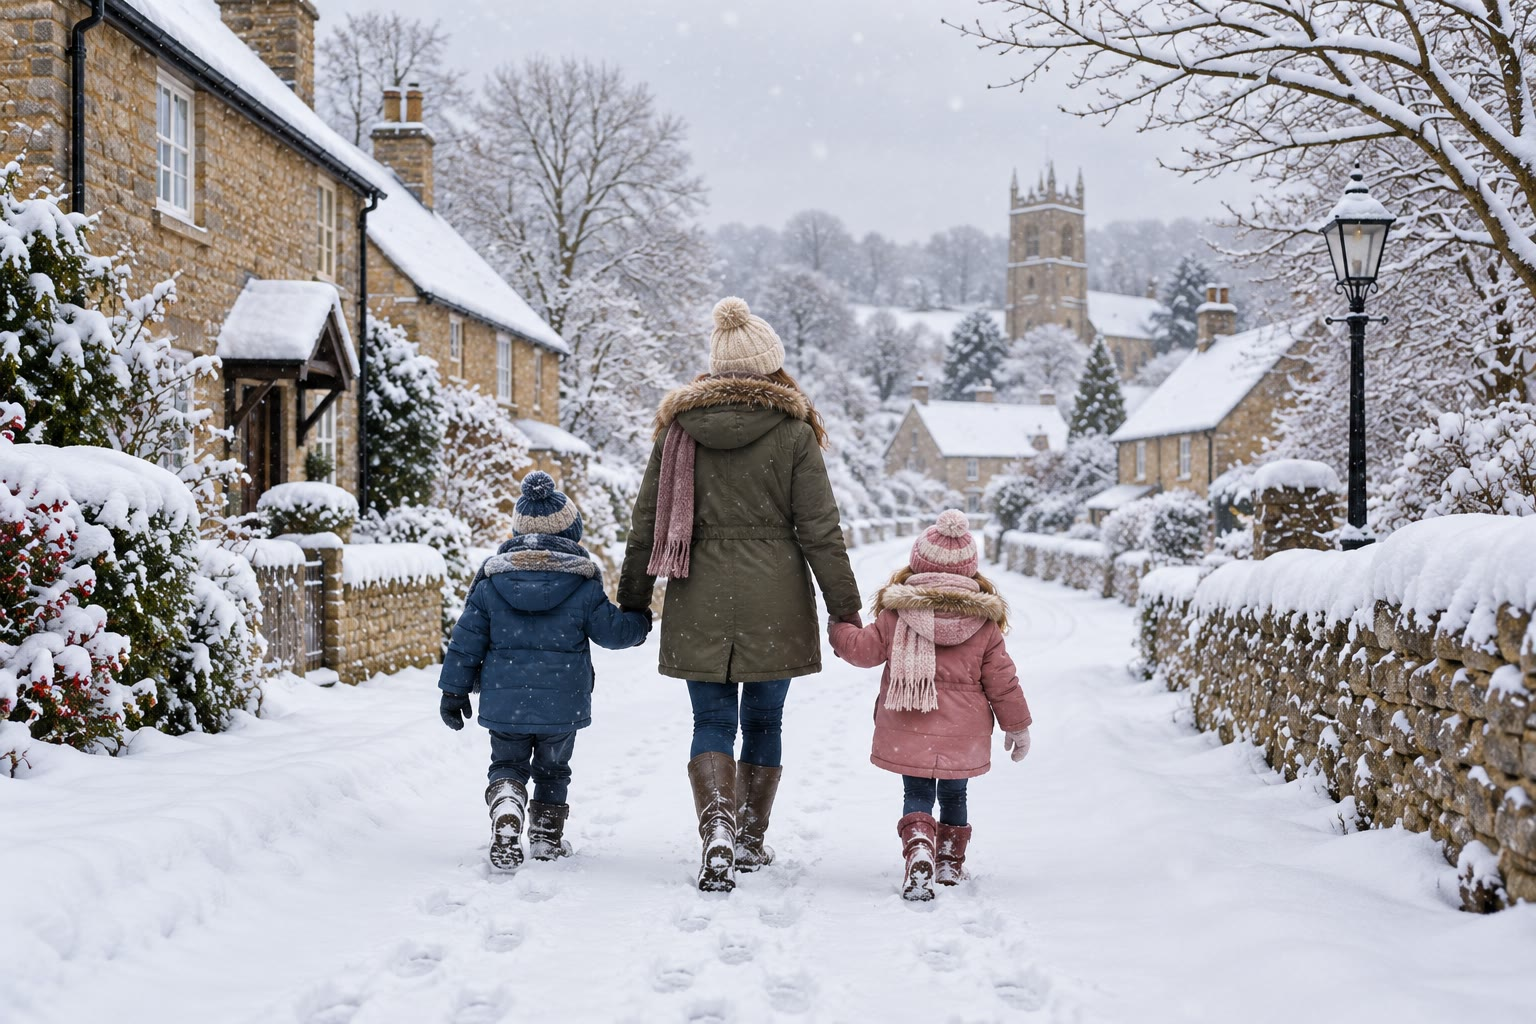
\includegraphics[width=\linewidth]{images/book1/ai/g1-snowy-street.jpg}

{\small Sneeuw en kou.}
\end{minipage}

\medskip
\begin{minipage}[b]{0.49\linewidth}\centering
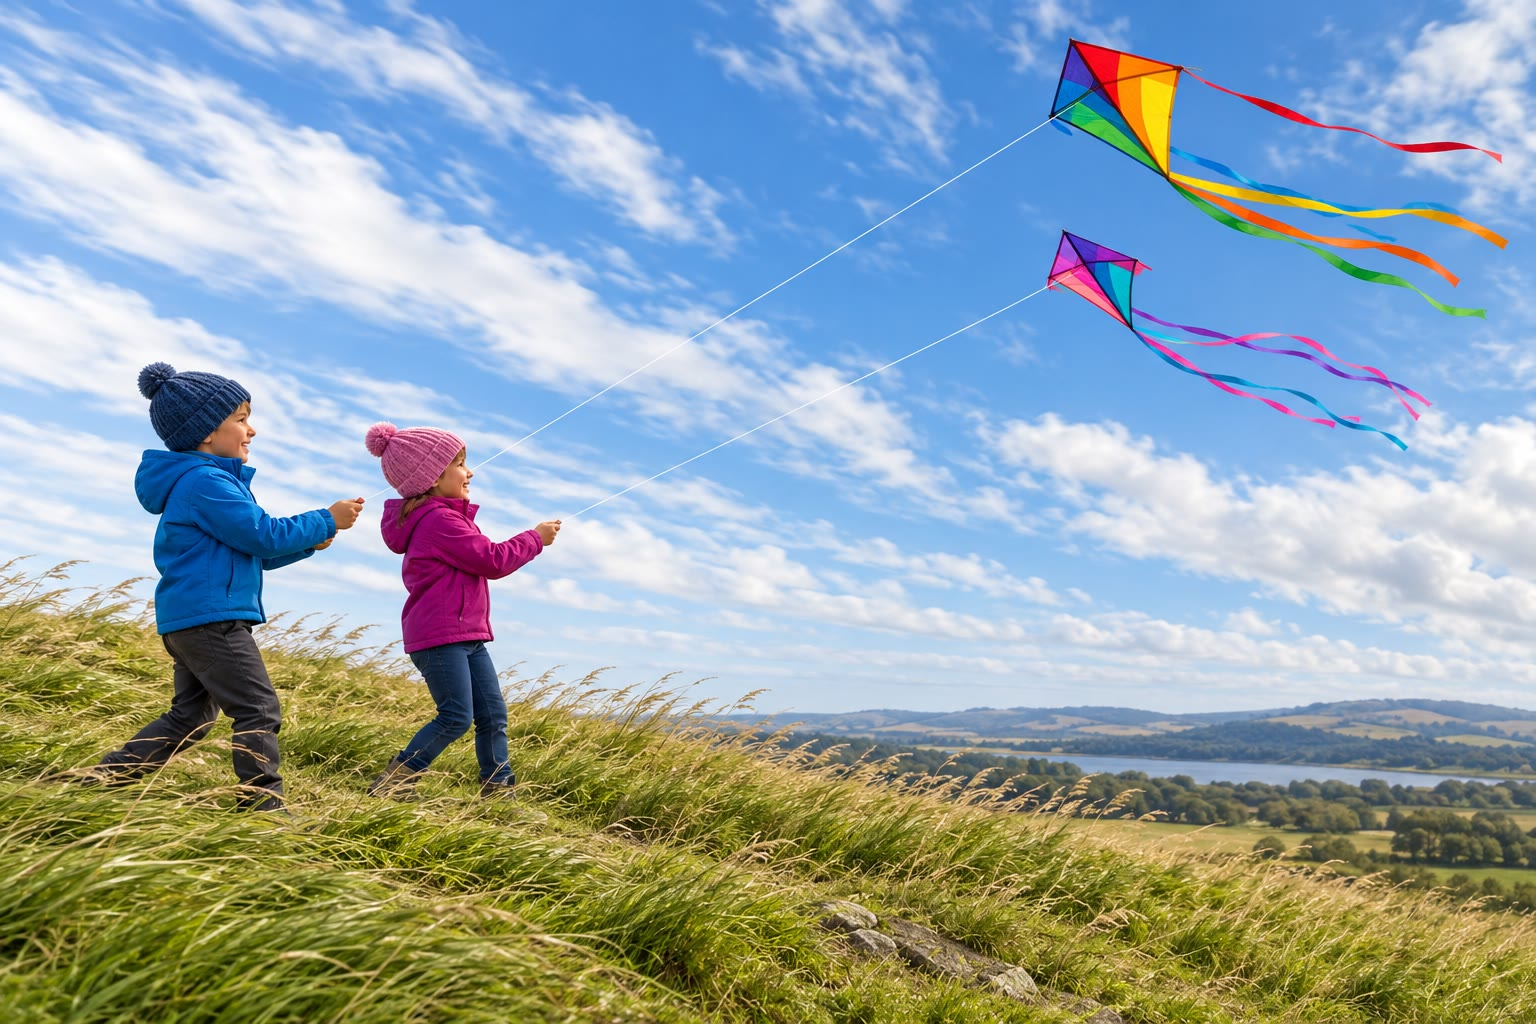
\includegraphics[width=\linewidth]{images/book1/ai/g1-windy-kites.jpg}

{\small Winderig: de vliegers vliegen.}
\end{minipage}\hfill
\begin{minipage}[b]{0.49\linewidth}\centering
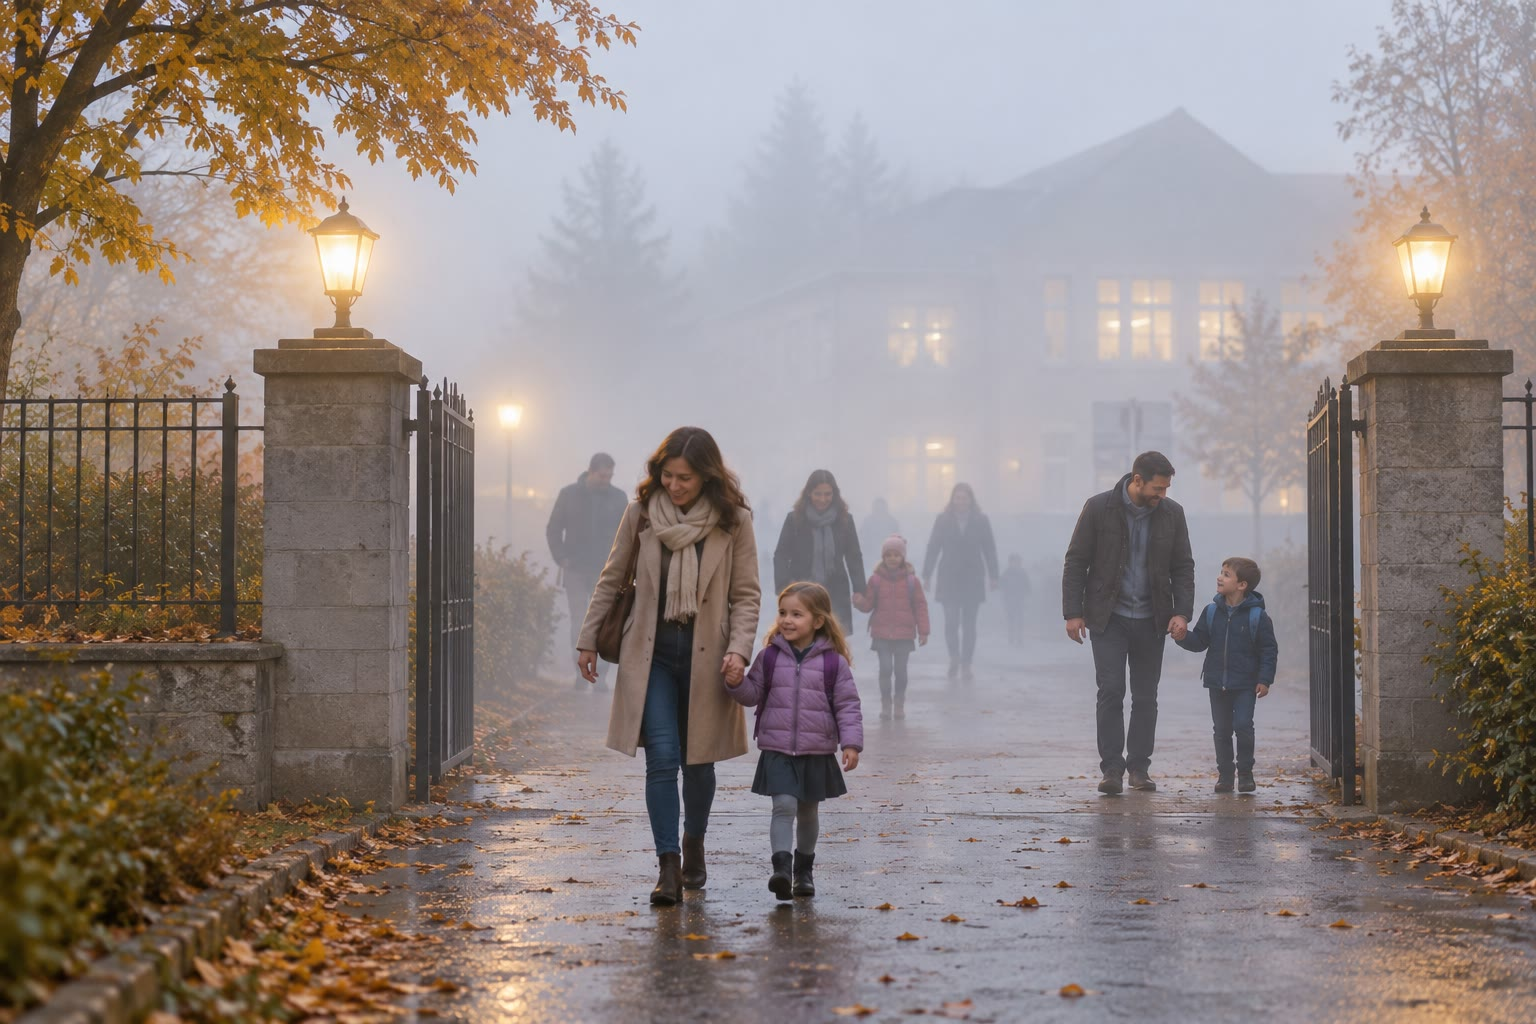
\includegraphics[width=\linewidth]{images/book1/ai/g1-foggy-school.jpg}

{\small Mist: we kunnen niet ver kijken.}
\end{minipage}
\end{omfigure}

\begin{example}[Mist]\label{ex:g1:watching-the-weather:fog}
Op sommige ochtenden lijkt de lucht zelf wit, en de bomen aan het eind van
de straat lijken te verdwijnen. Dat is mist. Mist is een wolk die de grond
raakt. Als het later op de dag warmer wordt, verdwijnt de mist vaak.
\end{example}

\section{Weersymbolen en de weerkalender}

Het \omterm{def:g1:watching-the-weather:weather}{weer} met woorden beschrijven duurt lang. Mensen die het \omterm{def:g1:watching-the-weather:weather}{weer}
bijhouden, gebruiken daarom kleine tekeningetjes: weersymbolen. Elk
symbool is makkelijk te tekenen en makkelijk te herkennen.

\begin{omfigure}
\begin{tikzpicture}[x=1cm, y=1cm]
  \foreach \i/\n/\t in {0/sun/zonnig, 1/suncloud/zon en wolken,
      2/cloud/bewolkt, 3/rain/regen, 4/shower/buien} {
    \pic[scale=1.25, transform shape] at (\i*2.6,0) {omwx=\n};
    \node[font=\small, align=center, text width=2.4cm] at (\i*2.6,-1.05) {\t};
  }
  \foreach \i/\n/\t in {0/snow/sneeuw, 1/storm/onweer, 2/fog/mist,
      3/wind/winderig} {
    \pic[scale=1.25, transform shape] at (\i*2.6+1.3,-2.6) {omwx=\n};
    \node[font=\small, align=center, text width=2.4cm] at (\i*2.6+1.3,-3.65) {\t};
  }
\end{tikzpicture}

{\small Negen weersymbolen. Bij onweer hoort een donkere wolk met een
bliksemflits; tussen de buien door schijnt af en toe de Zon.}
\end{omfigure}

\begin{definition}[Weerkalender]\label{def:g1:watching-the-weather:weather-chart}
Een \emph{weersymbool}\index{weersymbool} is een kleine tekening die één
soort \omterm{def:g1:watching-the-weather:weather}{weer} laat zien. Een \emph{weerkalender}\index{weerkalender} is een
tabel waarin we dag na dag opschrijven welk \omterm{def:g1:watching-the-weather:weather}{weer} we hebben gezien, met
weersymbolen.
\end{definition}

Een klas kan een hele week een \omterm{def:g1:watching-the-weather:weather-chart}{weerkalender} bijhouden. Elke ochtend, en
elke middag nog een keer, kijkt een kind naar buiten en tekent het symbool
in het goede vakje. We schrijven ook op of het warm of koud is.

\begin{omfigure}
\begin{tikzpicture}[x=1cm, y=1cm]
  \def\cw{1.9}
  \foreach \d [count=\i from 0] in {maandag, dinsdag, woensdag, donderdag,
      vrijdag, zaterdag, zondag}
    \node[font=\scriptsize\bfseries] at ({1.6+\i*\cw+\cw/2},0.35) {\d};
  \node[font=\scriptsize\bfseries, anchor=east] at (1.45,-0.5) {ochtend};
  \node[font=\scriptsize\bfseries, anchor=east] at (1.45,-1.5) {middag};
  \node[font=\scriptsize\bfseries, anchor=east, align=right] at (1.45,-2.35) {warm of\\koud?};
  \draw[black!60] (1.6,0) rectangle ({1.6+7*\cw},-2.7);
  \foreach \i in {1,...,6}
    \draw[black!60] ({1.6+\i*\cw},0.65) -- ({1.6+\i*\cw},-2.7);
  \draw[black!60] (1.6,0.65) -- ({1.6+7*\cw},0.65);
  \draw[black!60] (1.6,0.65) -- (1.6,0);
  \draw[black!60] ({1.6+7*\cw},0.65) -- ({1.6+7*\cw},0);
  \draw[black!60] (1.6,-1) -- ({1.6+7*\cw},-1);
  \draw[black!60] (1.6,-2) -- ({1.6+7*\cw},-2);
  \foreach \i/\m/\a/\w in {0/rain/rain/koud, 1/cloud/suncloud/koud,
      2/sun/sun/warm, 3/sun/suncloud/warm, 4/suncloud/shower/warm,
      5/fog/sun/warm, 6/cloud/rain/koud} {
    \pic[scale=0.8, transform shape] at ({1.6+\i*\cw+\cw/2},-0.5) {omwx=\m};
    \pic[scale=0.8, transform shape] at ({1.6+\i*\cw+\cw/2},-1.5) {omwx=\a};
    \node[font=\scriptsize] at ({1.6+\i*\cw+\cw/2},-2.35) {\w};
  }
\end{tikzpicture}

{\small De \omterm{def:g1:watching-the-weather:weather-chart}{weerkalender} die een klas een week lang in de lente bijhield.}
\label{fig:g1:watching-the-weather:chart}
\end{omfigure}

\begin{method}[Een weerkalender lezen]\label{met:g1:watching-the-weather:read}
Zo lees je een \omterm{def:g1:watching-the-weather:weather-chart}{weerkalender}:
\begin{enumerate}
  \item zoek de kolom van de dag die je wilt weten;
  \item kijk in de goede rij: de ochtend of de middag;
  \item zeg welk \omterm{def:g1:watching-the-weather:weather}{weer} het symbool laat zien.
\end{enumerate}
Wil je weten hoeveel dagen zonnig waren? Ga dan met je vinger langs een
rij en tel de zonnetjes.
\end{method}

\begin{example}[De kalender van de klas lezen]\label{ex:g1:watching-the-weather:read}
Op de kalender van deze klas was het maandagochtend regenachtig en koud.
Op woensdag was het de hele dag zonnig. Op zaterdag maakte de mist van de
ochtend 's middags plaats voor zon. Op de ochtenden van de week tekende de
klas op 2 dagen een zon: op woensdag en op donderdag.
\end{example}

\section{Het weer verandert}

Het \omterm{def:g1:watching-the-weather:weather}{weer} blijft niet hetzelfde. Het verandert in de loop van de dag, van
de ene dag op de andere, en in de loop van het jaar.

\begin{itemize}
  \item \textbf{In de loop van één dag.} Een grijze ochtend kan een zonnige
        middag worden. Een helderblauwe ochtend kan eindigen met onweer.
        Vroeg in de ochtend en 's nachts is het meestal koeler dan 's
        middags.
  \item \textbf{Van de ene dag op de andere.} Kijk naar de kalender van de
        klas: geen twee dagen van de week zijn precies hetzelfde.
  \item \textbf{In de loop van het jaar.} In de zomer zijn de dagen meestal
        warm, in de winter meestal koud; op veel plaatsen valt er alleen in
        de winter sneeuw. De natuurkundeboeken leggen uit waarom de
        seizoenen elk jaar terugkomen.
\end{itemize}

\begin{omfigure}
\begin{tikzpicture}[x=1cm, y=1cm]
  \draw[black!50, line width=0.8pt, -{Stealth[length=2.5mm]}] (0,0) -- (12.2,0);
  \foreach \x/\n/\t/\h in {0.9/fog/vroege ochtend/fris, 3.5/suncloud/ochtend/zacht,
      6.1/sun/middag/warm, 8.7/storm/late middag/warm met onweer,
      11.2/suncloud/avond/koeler} {
    \pic[scale=1.1, transform shape] at (\x,0.85) {omwx=\n};
    \fill[black!60] (\x,0) circle (1.5pt);
    \node[font=\scriptsize\bfseries, below] at (\x,-0.12) {\t};
    \node[font=\scriptsize, below] at (\x,-0.5) {\h};
  }
\end{tikzpicture}

{\small Eén zomerdag, van de ochtend tot de avond: het \omterm{def:g1:watching-the-weather:weather}{weer} verandert vijf
keer.}
\label{fig:g1:watching-the-weather:day}
\end{omfigure}

\begin{omfigure}
\begin{tikzpicture}[x=1cm, y=1cm]
  \foreach \i/\s/\c/\g/\w/\gr in {0/lente/green!55!black/pink!60/suncloud/green!35,
      1/zomer/green!45!black/green!50!black/sun/green!35,
      2/herfst/orange!80!black/orange!70/rain/green!25!brown!30,
      3/winter/black!55/white/snow/white} {
    \begin{scope}[shift={(\i*3.15,0)}]
      \draw[black!30, rounded corners=3pt, fill=ocBlue!6] (-1.4,-0.45) rectangle (1.4,3.05);
      \fill[\gr] (-1.4,-0.45) rectangle (1.4,0);
      \draw[black!25] (-1.4,0) -- (1.4,0);
      \fill[brown!60!black] (-0.09,0) rectangle (0.09,1.0);
      \draw[brown!60!black, line width=1.6pt] (0,0.75) -- (-0.5,1.35);
      \draw[brown!60!black, line width=1.6pt] (0,0.9) -- (0.45,1.45);
      \ifnum\i<3
        \fill[\c, opacity=0.85] (0,1.55) circle (0.72);
        \ifnum\i=0 \foreach \a in {20,80,140,200,260,320} \fill[\g] (0,1.55) ++(\a:0.45) circle (0.09); \fi
        \ifnum\i=2 \foreach \x/\y in {-0.9/0.15,0.7/0.3,0.95/0.1} \fill[\g] (\x,\y) circle (0.07); \fi
      \else
        \draw[white, line width=2.4pt] (-0.5,1.35) -- (-0.35,1.17);
        \draw[white, line width=2.4pt] (0.45,1.45) -- (0.3,1.27);
      \fi
      \pic[scale=0.8, transform shape] at (0.95,2.55) {omwx=\w};
      \node[font=\small\bfseries] at (0,-0.75) {\s};
    \end{scope}
  }
\end{tikzpicture}

{\small Dezelfde boom in de vier seizoenen: bloesem in de lente, dikke
groene bladeren in de zomer, vallende oranje bladeren in de herfst, kale
takken met sneeuw in de winter.}
\label{fig:g1:watching-the-weather:seasons}
\end{omfigure}

\begin{remark}[Waar de wind vandaan komt]\label{rem:g1:watching-the-weather:wind}
De wind kunnen we niet zien, maar wel wat hij doet. Een vlag, een windzak
of de rook uit een schoorsteen wordt door de wind weggeduwd: ze wijzen naar
waar de wind heen gaat, dus de wind komt van de andere kant.
\end{remark}

\begin{omfigure}
\begin{tikzpicture}[x=1cm, y=1cm]
  % ground
  \fill[green!30!omLithAlluv] (-0.4,-0.1) rectangle (8.4,0);
  % windsock on a pole
  \draw[black!70, line width=1.2pt] (1,0) -- (1,3.2);
  \fill[orange!85, draw=black!60] (1,3.15) -- (3.4,2.95) -- (3.4,2.55) -- (1,2.45) -- cycle;
  \fill[white] (1.6,3.1) -- (2.2,3.05) -- (2.2,2.5) -- (1.6,2.47) -- cycle;
  \fill[white] (2.8,3.0) -- (3.4,2.95) -- (3.4,2.55) -- (2.8,2.53) -- cycle;
  \draw[black!60] (1,3.15) -- (3.4,2.95) -- (3.4,2.55) -- (1,2.45);
  % flag
  \draw[black!70, line width=1.2pt] (5.4,0) -- (5.4,3.2);
  \fill[ocBlue!70, draw=black!60] (5.4,3.15) .. controls (6.0,3.3) and (6.4,2.9) .. (7.1,3.05)
     -- (7.1,2.35) .. controls (6.4,2.2) and (6.0,2.6) .. (5.4,2.45) -- cycle;
  % wind arrows
  \foreach \y in {1.0,1.6}
    \draw[omWxRain, line width=1.4pt, -{Stealth[length=3mm]}] (-0.3,\y) -- (0.7,\y);
  \node[font=\small, align=right, anchor=east] at (-0.45,1.3) {de wind\\komt van hier};
  \draw[black!60, -{Stealth[length=2mm]}] (4.1,2.75) -- (4.9,2.75);
  \node[font=\small, align=left, anchor=west] at (7.5,2.7) {vlag en windzak\\wijzen waar de\\wind heen gaat};
\end{tikzpicture}

{\small Een windzak en een vlag op een winderige dag. De wind waait van
links naar rechts.}
\end{omfigure}

\section{Waarom kijken we naar het weer?}

Veel mensen moeten weten wat voor \omterm{def:g1:watching-the-weather:weather}{weer} het wordt.
\begin{itemize}
  \item \textbf{Boeren} kijken naar de lucht voordat ze het hooi maaien:
        regen zou het bederven. In de lente zijn ze bang voor een nacht met
        vorst, die de jonge plantjes kan doden.
  \item \textbf{Zeelui en vissers} letten op de wind: een harde wind maakt
        hoge golven, en dan blijven de boten in de haven.
  \item \textbf{Piloten} moeten van mist, onweer en wind weten voordat een
        vliegtuig opstijgt.
  \item \textbf{Een klas} die een uitstapje naar het bos maakt, wil weten
        of ze regenjassen of zonnehoedjes moet meenemen.
\end{itemize}
Elke dag houden mensen die we meteorologen noemen het \omterm{def:g1:watching-the-weather:weather}{weer} over de hele
wereld in de gaten. Op de radio, op de televisie of op een telefoon
vertellen ze ons hoe het \omterm{def:g1:watching-the-weather:weather}{weer} de komende dagen waarschijnlijk wordt.

\begin{example}[Tekens aan de hemel]\label{ex:g1:watching-the-weather:signs}
Lang voordat er radio's en telefoons waren, leerden mensen de hemel te
lezen. Als kleine witte wolkjes 's middags uitgroeien tot hoge donkere
torens, komt er een bui of onweer aan. Als de wind draait en de hemel
langzaam vol raakt met een grijze sluier, volgt er vaak een paar uur later
regen. Deze tekens kloppen niet altijd, maar ze zijn vaak nuttig.
\end{example}

\section{Je kleden naar het weer}

Nu kan Lena haar vraag beantwoorden. Het regent en het is koud, dus trekt
ze haar regenjas en haar laarzen aan. Morgen is het \omterm{def:g1:watching-the-weather:weather}{weer} misschien anders,
en dan kiest ze opnieuw.

\begin{omfigure}
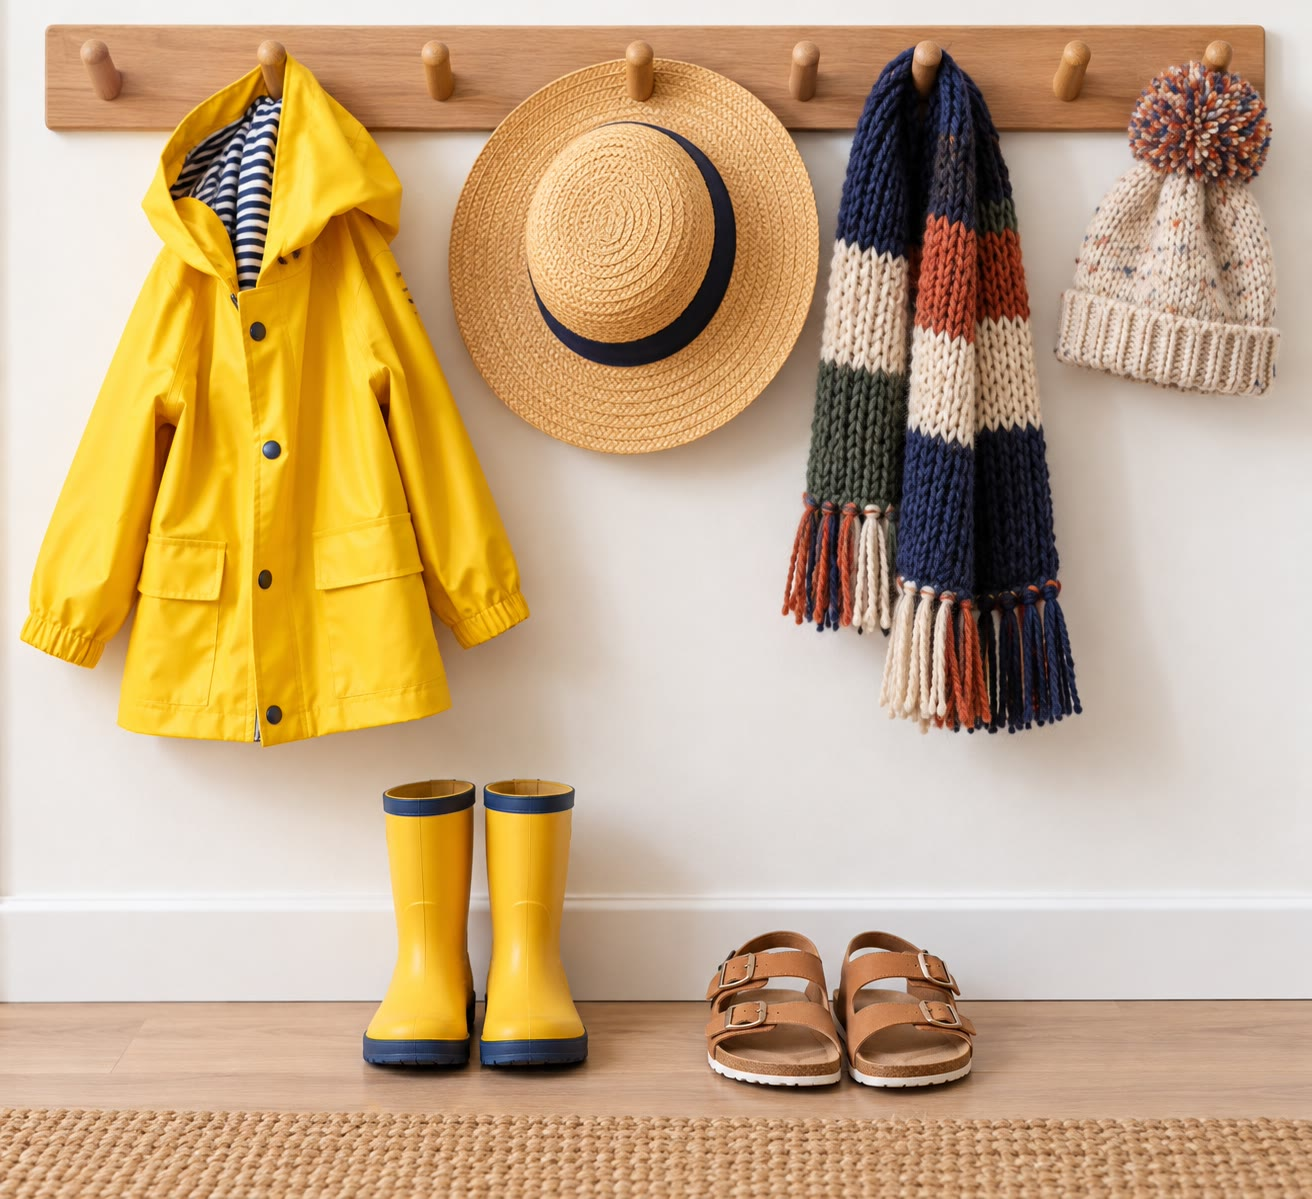
\includegraphics[width=0.66\linewidth]{images/book1/ai/g1-coat-pegs.jpg}

{\small Kleren voor elk soort \omterm{def:g1:watching-the-weather:weather}{weer}: een regenjas, een zonnehoed, een sjaal
en een warme muts, laarzen en sandalen.}
\end{omfigure}

\begin{method}[Kleren kiezen voor het weer]\label{met:g1:watching-the-weather:clothes}
Kijk naar de hemel en voel de lucht, en dan:
\begin{itemize}
  \item regen of buien: een regenjas of een paraplu, en laarzen;
  \item kou of sneeuw: een warme jas, een sjaal, een muts en handschoenen;
  \item felle zon en hitte: een zonnehoed, lichte kleren, en water om te
        drinken;
  \item wind: een jas die goed sluit; een paraplu helpt dan niet veel.
\end{itemize}
\end{method}

\begin{safety}
\textbf{Kijk nooit recht in de Zon}, zelfs niet heel even, en nooit door
een bril, een verrekijker of een camera: je ogen kunnen er voor altijd
beschadigd door raken. Bij onweer blijf je binnen of in een auto, ver van
hoge bomen en van water, en wacht je tot het onweer voorbij is.
\end{safety}

\section{Oefeningen}

\begin{exercise}[$\star$]\label{exo:g1:watching-the-weather:1}
Teken het symbool voor elk soort \omterm{def:g1:watching-the-weather:weather}{weer}: zonnig; regen; sneeuw; bewolkt.
\end{exercise}

\begin{exercise}[$\star$]\label{exo:g1:watching-the-weather:2}
Wat voor \omterm{def:g1:watching-the-weather:weather}{weer} is het op elk van de vier plaatjes van de paragraaf ``Wat is
het \omterm{def:g1:watching-the-weather:weather}{weer}?''? Gebruik voor elk plaatje één of twee woorden.
\end{exercise}

\begin{exercise}[$\star$]\label{exo:g1:watching-the-weather:3}
Kijk naar de \omterm{def:g1:watching-the-weather:weather-chart}{weerkalender} van de klas. Wat voor \omterm{def:g1:watching-the-weather:weather}{weer} was het op
dinsdagochtend? Op vrijdagmiddag? Op zondagmiddag?
\end{exercise}

\begin{exercise}[$\star$]\label{exo:g1:watching-the-weather:4}
Op welke dag was het volgens de \omterm{def:g1:watching-the-weather:weather-chart}{weerkalender} van de klas zowel 's ochtends
als 's middags zonnig?
\end{exercise}

\begin{exercise}[$\star$]\label{exo:g1:watching-the-weather:5}
Zoek bij elk kledingstuk het \omterm{def:g1:watching-the-weather:weather}{weer} dat erbij past: een zonnehoed; laarzen
en een regenjas; een sjaal en handschoenen. De soorten weer zijn: koud met
sneeuw; warm en zonnig; regen.
\end{exercise}

\begin{exercise}[$\star$]\label{exo:g1:watching-the-weather:6}
Lena zegt: ``Kijk, de vlag wappert!'' Wat voor \omterm{def:g1:watching-the-weather:weather}{weer} is het?
\end{exercise}

\begin{exercise}[$\star$]\label{exo:g1:watching-the-weather:7}
Waar of niet waar? Leg uit.
\begin{enumerate}
  \item 's Ochtends en 's middags is het \omterm{def:g1:watching-the-weather:weather}{weer} altijd hetzelfde.
  \item Mist is een wolk die de grond raakt.
  \item De regel ``kijk nooit naar de Zon, ook niet met één oog'' is een goede regel.
\end{enumerate}
\end{exercise}

\begin{exercise}[$\star\star$]\label{exo:g1:watching-the-weather:8}
Tel op de \omterm{def:g1:watching-the-weather:weather-chart}{weerkalender} van de klas de middagen met regen of buien. Tel de
koude dagen. Was de week vooral warm of vooral koud?
\end{exercise}

\begin{exercise}[$\star\star$]\label{exo:g1:watching-the-weather:9}
Dit zag Sam die dag vanuit zijn raam: 's ochtends een grijze lucht; rond
het middageten druppels op het raam; 's avonds een blauwe lucht met een
paar wolkjes. Teken de drie weersymbolen in de goede volgorde.
\end{exercise}

\begin{exercise}[$\star\star$]\label{exo:g1:watching-the-weather:10}
Op het plaatje van de windzak en de vlag komt de wind van links. Op een
andere dag wijst een vlag naar links. Van welke kant komt de wind op die
dag?
\end{exercise}

\begin{exercise}[$\star\star$]\label{exo:g1:watching-the-weather:11}
Kijk naar de tekening van dezelfde boom in de vier seizoenen. In welk
seizoen heeft de boom geen bladeren? In welk seizoen heeft hij bloesem?
Welk \omterm{def:g1:watching-the-weather:weather-chart}{weersymbool} staat bij de winter, en waarom past het bij dat seizoen?
\end{exercise}
